% $Id: comp_desdoc.tex,v 1.4 2002/08/18 23:56:21 eschwab Exp $

\documentclass[]{article}

\usepackage{epsf}
\usepackage{html}
\usepackage[T1]{fontenc}
\usepackage[dvips]{graphics,color}

\textwidth 6.5in
\textheight 8.5in
\addtolength{\oddsidemargin}{-.75in}

\begin{document}

\bodytext{BGCOLOR=white LINK=#083194 VLINK=#21004A}

\begin{titlepage}

\begin{center}
{\Large Earth System Modeling Framework } \\
\vspace{.25in}
{\Large {\bf <Module, Library, Component or Model Name> Design}} \\
\vspace{.25in}
{\large {\it Authors}} \\
\vspace{.25in}
{Month DD, CCYY}
\vspace{.5in}
\end{center}

\begin{latexonly}
\vspace{5.5in}
\begin{tabular}{p{5in}p{.9in}}
\hrulefill \\
\noindent {\bf NASA Earth Science Technology Office} \\
\noindent Computational Technologies Project \\
\noindent CAN 00-OES-01 \\
\noindent http://www.esmf.ucar.edu \\
\end{tabular}
\end{latexonly}

\end{titlepage}

\tableofcontents

\newpage
\section{Synopsis}
% $Id: comp_syn.tex,v 1.6 2008/04/05 03:37:54 cdeluca Exp $
%
% Earth System Modeling Framework
% Copyright 2002-2008, University Corporation for Atmospheric Research, 
% Massachusetts Institute of Technology, Geophysical Fluid Dynamics 
% Laboratory, University of Michigan, National Centers for Environmental 
% Prediction, Los Alamos National Laboratory, Argonne National Laboratory, 
% NASA Goddard Space Flight Center.
% Licensed under the University of Illinois-NCSA License.

%\section{Synopsis}

<Brief synopsis of component or library.>


%\section{Algorithmic Description}
%% $Id: comp_alg.tex,v 1.6 2008/04/05 03:37:53 cdeluca Exp $
%
% Earth System Modeling Framework
% Copyright 2002-2008, University Corporation for Atmospheric Research, 
% Massachusetts Institute of Technology, Geophysical Fluid Dynamics 
% Laboratory, University of Michigan, National Centers for Environmental 
% Prediction, Los Alamos National Laboratory, Argonne National Laboratory, 
% NASA Goddard Space Flight Center.
% Licensed under the University of Illinois-NCSA License.

%\section{Algorithmic Description}

<Description of the continuous and discrete scientific algorithms used
in the software.  May reference rather than describe algorithms explicitly.>





\section{Object Model}
$Id: comp_obj.tex,v 1.2 2002/10/14 21:54:17 cdeluca Exp $
%
% Earth System Modeling Framework
% Copyright 2002-2003, University Corporation for Atmospheric Research, 
% Massachusetts Institute of Technology, Geophysical Fluid Dynamics 
% Laboratory, University of Michigan, National Centers for Environmental 
% Prediction, Los Alamos National Laboratory, Argonne National Laboratory, 
% NASA Goddard Space Flight Center.
% Licensed under the GPL.

%\section{Object Model}

<Descriptive text>

\begin{center}
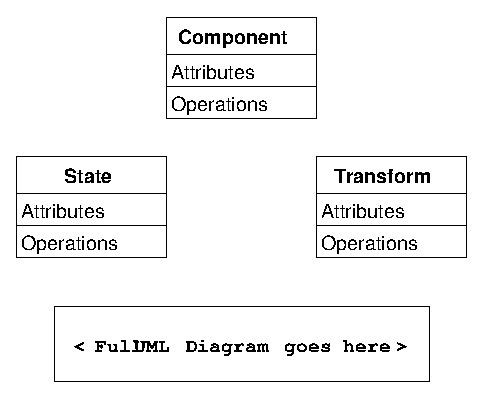
\includegraphics{comp_obj.EPS}
   
Figure 1.  Comp Class Diagram
   
\end{center}


\section{Global Parameters and Definitions}
$Id: comp_param.tex,v 1.3 2006/11/16 05:20:53 cdeluca Exp $
%
% Earth System Modeling Framework
% Copyright 2002-2008, University Corporation for Atmospheric Research, 
% Massachusetts Institute of Technology, Geophysical Fluid Dynamics 
% Laboratory, University of Michigan, National Centers for Environmental 
% Prediction, Los Alamos National Laboratory, Argonne National Laboratory, 
% NASA Goddard Space Flight Center.
% Licensed under the University of Illinois-NCSA License.

%\section{Global Parameters and Definitions}

<List F90 and C++ parameters and \#define constants>


\section{<Name1> Design}

\subsection{Description}
% $Id: class_desc.tex,v 1.3 2002/10/14 21:54:05 cdeluca Exp $
%
% Earth System Modeling Framework
% Copyright 2002-2003, University Corporation for Atmospheric Research, 
% Massachusetts Institute of Technology, Geophysical Fluid Dynamics 
% Laboratory, University of Michigan, National Centers for Environmental 
% Prediction, Los Alamos National Laboratory, Argonne National Laboratory, 
% NASA Goddard Space Flight Center.
% Licensed under the GPL.

%\subsection{Description}

<Describe class function and relation to other classes.>


\subsection{Design}
% $Id: class_design.tex,v 1.1 2001/12/13 20:03:39 cdeluca Exp $

\subsection{Design}

<Describe strategy for overall class design.>

%\subsubsection{Class Definition}
% $Id: class_def.tex,v 1.2 2002/07/25 17:11:11 eschwab Exp $

%\subsubsection{Class Definition}

<Show internal attributes and methods of derived type, structure or class.

 This definition can be expressed using a general language like UML 
 (see, e.g. ``The Unified Modeling Language Reference Manual,'' 
 Rumbaugh et. al. 1999) or using constructs from a specific language like 
 Fortran.>


\subsubsection{Restrictions}
% $Id: class_rest.tex,v 1.4 2006/11/16 05:20:53 cdeluca Exp $
%
% Earth System Modeling Framework
% Copyright 2002-2008, University Corporation for Atmospheric Research, 
% Massachusetts Institute of Technology, Geophysical Fluid Dynamics 
% Laboratory, University of Michigan, National Centers for Environmental 
% Prediction, Los Alamos National Laboratory, Argonne National Laboratory, 
% NASA Goddard Space Flight Center.
% Licensed under the University of Illinois-NCSA License.

%\subsubsection{Restrictions}

<List class restrictions due to design or implementation strategies.>







\subsubsection{Class Definition}
% $Id: class_def.tex,v 1.2 2002/07/25 17:11:11 eschwab Exp $

%\subsubsection{Class Definition}

<Show internal attributes and methods of derived type, structure or class.

 This definition can be expressed using a general language like UML 
 (see, e.g. ``The Unified Modeling Language Reference Manual,'' 
 Rumbaugh et. al. 1999) or using constructs from a specific language like 
 Fortran.>


\subsubsection{Restrictions}
% $Id: class_rest.tex,v 1.4 2006/11/16 05:20:53 cdeluca Exp $
%
% Earth System Modeling Framework
% Copyright 2002-2008, University Corporation for Atmospheric Research, 
% Massachusetts Institute of Technology, Geophysical Fluid Dynamics 
% Laboratory, University of Michigan, National Centers for Environmental 
% Prediction, Los Alamos National Laboratory, Argonne National Laboratory, 
% NASA Goddard Space Flight Center.
% Licensed under the University of Illinois-NCSA License.

%\subsubsection{Restrictions}

<List class restrictions due to design or implementation strategies.>


\section{<Name1> F90 Interface}

\subsection{Use and Examples}
% $Id: class_fex.tex,v 1.7 2008/04/05 03:37:52 cdeluca Exp $
%
% Earth System Modeling Framework
% Copyright 2002-2008, University Corporation for Atmospheric Research, 
% Massachusetts Institute of Technology, Geophysical Fluid Dynamics 
% Laboratory, University of Michigan, National Centers for Environmental 
% Prediction, Los Alamos National Laboratory, Argonne National Laboratory, 
% NASA Goddard Space Flight Center.
% Licensed under the University of Illinois-NCSA License.

%\subsection{F90 Use and Examples}

<Detailed examples of F90 usage of the class.>


\subsection{Parameters and Definitions}
% $Id: class_fparam.tex,v 1.5 2007/03/31 05:50:45 cdeluca Exp $
%
% Earth System Modeling Framework
% Copyright 2002-2007, University Corporation for Atmospheric Research, 
% Massachusetts Institute of Technology, Geophysical Fluid Dynamics 
% Laboratory, University of Michigan, National Centers for Environmental 
% Prediction, Los Alamos National Laboratory, Argonne National Laboratory, 
% NASA Goddard Space Flight Center.
% Licensed under the University of Illinois-NCSA License.

%\subsection{Parameters}

\begin{description}

\item [<ITEM1>] <Description of ITEM1.>

\item [<ITEM2>] <Description of ITEM2.>

\end{description}










%\subsection{Class API}
% $Id: class_fapi.tex,v 1.1 2002/11/13 22:08:47 ekluz Exp $
%
% Earth System Modeling Framework
% Copyright 2002-2003, University Corporation for Atmospheric Research, 
% Massachusetts Institute of Technology, Geophysical Fluid Dynamics 
% Laboratory, University of Michigan, National Centers for Environmental 
% Prediction, Los Alamos National Laboratory, Argonne National Laboratory, 
% NASA Goddard Space Flight Center.
% Licensed under the GPL.

%\subsection{Parameters}

\begin{description}

\item [<ITEM1>] <Description of ITEM1.>

\item [<ITEM2>] <Description of ITEM2.>

\end{description}










\section{<Name1> C++ Interface}

\subsection{Use and Examples}
% $ Id: $
%
% Earth System Modeling Framework
% Copyright 2002-2003, University Corporation for Atmospheric Research, 
% Massachusetts Institute of Technology, Geophysical Fluid Dynamics 
% Laboratory, University of Michigan, National Centers for Environmental 
% Prediction, Los Alamos National Laboratory, Argonne National Laboratory, 
% NASA Goddard Space Flight Center.
% Licensed under the GPL.

%\subsection{C++ Use and Examples}

<Detailed examples of C++ usage of the class.>









\subsection{Parameters and Definitions}
% $Id: class_ccparam.tex,v 1.5 2008/04/05 03:37:52 cdeluca Exp $
%
% Earth System Modeling Framework
% Copyright 2002-2008, University Corporation for Atmospheric Research, 
% Massachusetts Institute of Technology, Geophysical Fluid Dynamics 
% Laboratory, University of Michigan, National Centers for Environmental 
% Prediction, Los Alamos National Laboratory, Argonne National Laboratory, 
% NASA Goddard Space Flight Center.
% Licensed under the University of Illinois-NCSA License.

%\subsection{Parameters}

\begin{description}

\item [<ITEM1>] <Description of ITEM1.>

\item [<ITEM2>] <Description of ITEM2.>

\end{description}









%\subsection{Class API}
% $ Id: $
%
% Earth System Modeling Framework
% Copyright 2002-2003, University Corporation for Atmospheric Research, 
% Massachusetts Institute of Technology, Geophysical Fluid Dynamics 
% Laboratory, University of Michigan, National Centers for Environmental 
% Prediction, Los Alamos National Laboratory, Argonne National Laboratory, 
% NASA Goddard Space Flight Center.
% Licensed under the GPL.

%\subsection{C++ Use and Examples}

<Detailed examples of C++ usage of the class.>









\section{<Name2> Design}

% Subsections same as <Name1> Design ...

\section{Review Status}

\noindent{\bf Design Review} \\

\begin{tabular}{r p{1.3in} p{2in}}
{\bf Review Date:} & <Date> \\ \\
{\bf Reviewers:}   & Reviewer           & <Institution> \\
                   & Reviewer           & <Institution> \\
                   & Reviewer           & <Institution>
\end{tabular}

%\section{Glossary}
% $Id: comp_glos.tex,v 1.4 2006/11/16 05:20:53 cdeluca Exp $
%
% Earth System Modeling Framework
% Copyright 2002-2008, University Corporation for Atmospheric Research, 
% Massachusetts Institute of Technology, Geophysical Fluid Dynamics 
% Laboratory, University of Michigan, National Centers for Environmental 
% Prediction, Los Alamos National Laboratory, Argonne National Laboratory, 
% NASA Goddard Space Flight Center.
% Licensed under the University of Illinois-NCSA License.

% USAGE NOTE:
%
% The first use of a term in the text of a document can be 
% linked to the corresponding glossary item using the item label.
% 
% For example,
%
% Original document text: code must include item1
%
% Linked to glossary:     code must include \htmlref{item1}{glos:item1}
%
% The link will appear in the html version of the document.
% The print version of the document will appear unchanged.

\begin{description}

\item [item1] \label{glos:item1} <Definition of item1.>

\item [item2] \label{glos:item2} <Definition of item2.>

\end{description}










%\section{Bibliography}
\bibliography{comp} 
\bibliographystyle{plain}
\addcontentsline{toc}{section}{Bibliography}

\end{document}











